\documentclass[t, aspectratio=169]{beamer}
\usepackage{fontspec}
\usepackage{amsmath,amssymb}
\usepackage{tikz}
\usepackage{array}
\usepackage{booktabs}
\newcolumntype{R}[1]{>{\raggedright\arraybackslash}p{#1}}
\usepackage{url}
\usepackage{fancyvrb}
\usetikzlibrary{arrows.meta, positioning, fit, shapes.geometric, calc}

% --- Lề nội dung (theo mẫu HUST) ---
\def\slideContentLeftMargin{0.5cm}
\def\slideContentRightMargin{0.7cm}
\def\hustHeaderHeight{1.1cm}
\def\slideContentBotMargin{3.5cm}

\usepackage[blue, 169]{beamerthemeHUST}

\renewcommand{\titlePageTitleX}{-0.5cm}
\renewcommand{\titlePageTitleY}{-0.5cm}
\renewcommand{\hustTitleAlign}{\alignLeft}
\renewcommand{\hustSubtitleAlign}{\alignLeft}
\renewcommand{\hustAuthorAlign}{\alignLeft}
\renewcommand{\hustInstAlign}{\alignLeft}

% Bỏ khoảng đệm phía trên mà theme thêm sau tiêu đề frame
\setlength{\abovedisplayskip}{2pt}
\renewcommand{\slideContentTopPadding}{0cm}

% Trang section: đưa tiêu đề xuống giữa trang
\renewcommand{\hustsectionpage}[1]{{
  \setbeamertemplate{background}{\includegraphics[width=\paperwidth,height=\paperheight]{\hustbg{section}}}
  \begin{frame}[plain]
    \vspace*{3.4cm}\centering \Huge \textcolor{white}{\textbf{#1}}
  \end{frame}
}}

% --- Màu và macro dùng lại ---
\definecolor{warn}{HTML}{C0392B}
\definecolor{wait}{HTML}{D9822B}
\definecolor{okgreen}{HTML}{005a8c}
\definecolor{softblue}{HTML}{E6F0F6}
\definecolor{softwarn}{HTML}{FBEAE5}

\newcommand{\badge}[2]{\tikz[baseline=(b.base)]\node[fill=#1, text=white, rounded corners=2pt, inner xsep=3pt, inner ysep=1.5pt, font=\bfseries\tiny] (b) {#2};}
\newcommand{\bDone}{\badge{hustprimary}{Đã xong}}
\newcommand{\bHW}{\badge{wait}{Chờ phần cứng}}
\newcommand{\bTwo}{\badge{gray}{Sprint 2}}
\newcommand{\bThree}{\badge{gray}{Sprint 3}}
\newcommand{\TODO}[1]{\textcolor{red}{\textbf{[#1]}}}
\newcommand{\step}[2]{\par\noindent\hangindent=0.55cm\hangafter=1 {\color{hustprimary}\textbf{#1}}\hspace{0.15cm}#2\par\vspace{1.6mm}}
\newcommand{\nfrbox}[4]{%
  \node[anchor=north west, fill=hustprimary, text=white, font=\small\bfseries, text width=7.0cm, inner xsep=6pt, inner ysep=4pt] (nfrt) at (#1,#2) {#3};
  \node[anchor=north west, fill=softblue, text=black, font=\small, inner xsep=6pt, inner ysep=5pt] at (nfrt.south west) {\parbox[t][2.2cm][t]{6.9cm}{\raggedright #4}};}
\newcommand{\hl}[1]{\textcolor{hustprimary}{\textbf{#1}}}
\setbeamercolor{terminal}{bg=black!85, fg=white}
\definecolor{termok}{HTML}{7EE787}
\definecolor{termwarn}{HTML}{FFA657}
\newcommand{\tok}[1]{\textcolor{termok}{#1}}
\newcommand{\twarn}[1]{\textcolor{termwarn}{#1}}
\newcommand{\termlabel}[1]{{\footnotesize\hl{#1}}\par\vspace{0.6mm}}
\newcommand{\cnum}[1]{\tikz[baseline=(c.base)]\node[circle, fill=hustprimary, text=white, inner sep=0.9pt, font=\scriptsize\bfseries] (c) {#1};}

\setbeamerfont{block title}{size=\small}
\setbeamercolor{block title}{bg=hustprimary, fg=white}
\setbeamercolor{block body}{bg=softblue, fg=black}
\setbeamercolor{block title alerted}{bg=warn, fg=white}
\setbeamercolor{block body alerted}{bg=softwarn, fg=black}
\setbeamertemplate{itemize item}{\color{hustprimary}$\bullet$}
\setbeamertemplate{itemize subitem}{\color{hustprimary}$\circ$}

\tikzset{
  box/.style={draw=hustprimary, fill=softblue, rounded corners=3pt, align=center, font=\footnotesize, minimum height=1cm, text width=2.7cm, thick},
  boxdone/.style={box, fill=hustprimary!15},
  boxwait/.style={box, draw=wait, fill=wait!10, dashed},
  arr/.style={-{Stealth[length=2mm]}, thick, hustprimary},
  arrwait/.style={-{Stealth[length=2mm]}, thick, wait, dashed},
  lbl/.style={font=\tiny, align=center, text=black!75},
}

\title{Noise Monitor}
\subtitle{Hệ thống giám sát tiếng ồn trong phòng ngủ \\ Báo cáo tiến độ lần 1 (Checkpoint 1) — Nhóm 14 · PAN}
\author{\texorpdfstring{Nguyễn Ngọc Tuấn Anh – 202400029 \\ Nguyễn Hải Yến Nhi – 202400064 \\ Nguyễn Phong – 202400066}{Nguyễn Ngọc Tuấn Anh – 202400029, Nguyễn Hải Yến Nhi – 202400064, Nguyễn Phong – 202400066}}
\institute{Học phần: IoT và ứng dụng (IT4735) · Mã lớp: 175680 \\ Giảng viên: Đặng Tuấn Linh}

\begin{document}

\husttitlepage

\begin{frame}{Nội dung trình bày}
  \tableofcontents[hideallsubsections]
\end{frame}

\resetPageCount
\showPageNumber
\useStyleHustFull
\useThinBar

% =====================================================================
\section{Giới thiệu}
\hustsectionpage{1. Giới thiệu}

\begin{frame}{Noise Monitor là gì?}
  \large
  Thiết bị đặt trong phòng ngủ, \hl{đo mức tiếng ồn liên tục cả đêm}, xử lý ngay trên ESP32 và \hl{chỉ gửi số liệu (không ghi âm)} lên server; người dùng xem lại trên web.

  \vspace{1.3cm}
  \centering
  \begin{tikzpicture}[node distance=0.8cm]
    \tikzset{big/.style={box, font=\normalsize, minimum height=2.4cm}}
    \node[big, text width=2.3cm] (mic) {Micro\\MAX4466};
    \node[big, right=of mic, text width=2.5cm] (esp) {ESP32\\\small xử lý tại chỗ};
    \node[big, right=of esp, text width=2.3cm] (srv) {Server};
    \node[big, right=of srv, text width=2.3cm] (web) {Web};
    \draw[arr] (mic) -- (esp);
    \draw[arr] (esp) -- (srv);
    \draw[arr] (srv) -- (web);
    \node[font=\footnotesize, text=black!75, anchor=north, yshift=-2mm] at ($(esp.south east)!0.5!(srv.south west)$) {chỉ gửi số liệu, không gửi âm thanh thô};
  \end{tikzpicture}
\end{frame}

\begin{frame}{Thành viên nhóm}
  \small
  \renewcommand{\arraystretch}{1.7}
  \begin{tabular}{@{}R{3.5cm}R{1.9cm}R{2.9cm}R{5.4cm}@{}}
    \toprule
    \textbf{Họ tên} & \textbf{MSSV} & \textbf{GitHub} & \textbf{Phụ trách chính} \\
    \midrule
    Nguyễn Ngọc Tuấn Anh & 202400029 & nnta301 & Quy trình repo \& CI, backend API, tích hợp hệ thống \\
    Nguyễn Hải Yến Nhi & 202400064 & nhiyen26 & Contract dữ liệu telemetry, dashboard web \\
    Nguyễn Phong & 202400066 & nguyenphongg233 & Firmware ESP32, simulator dữ liệu \\
    \bottomrule
  \end{tabular}
\end{frame}

\begin{frame}{Vấn đề và người dùng mục tiêu}
  \footnotesize
  \begin{columns}[T]
    \begin{column}{0.53\textwidth}
      \textbf{\hl{Người dùng:}} sinh viên ở KTX/phòng trọ; người sống gần đường lớn hoặc khu đông dân.

      \vspace{1mm}
      \textbf{\hl{Vấn đề:}} tiếng ồn ban đêm (xe cộ, hàng xóm, sinh hoạt chung phòng) làm gián đoạn giấc ngủ, nhưng người ngủ không biết ồn lúc mấy giờ, kéo dài bao lâu, lặp lại ra sao; sáng dậy chỉ còn cảm giác ``đêm qua ồn''.

      \vspace{1mm}
      \textbf{\hl{Cách hiện có \& hạn chế:}}
      \begin{itemize}\setlength{\itemsep}{0pt}
        \item App điện thoại ghi âm cả đêm: lộ riêng tư người cùng phòng, tốn pin, phải để máy cạnh giường.
        \item Máy đo âm thanh cầm tay: chỉ đo tức thời, không lưu lịch sử.
      \end{itemize}
    \end{column}
    \begin{column}{0.44\textwidth}
      \begin{block}{Nhu cầu $\rightarrow$ giải pháp}
        \footnotesize Thiết bị rẻ, đặt cố định, đo liên tục, \textbf{không ghi âm}, xem lại mức ồn theo thời gian $\rightarrow$ dữ liệu khách quan để điều chỉnh (đổi vị trí giường, đóng cửa sổ, nút tai, trao đổi với hàng xóm/chủ trọ).
      \end{block}
      \begin{alertblock}{Phạm vi}
        \footnotesize Đo mức tín hiệu \emph{tương đối} (P2P, đơn vị ADC), không phải dB. Không nhận dạng loại âm thanh. Không đánh giá chất lượng giấc ngủ.
      \end{alertblock}
    \end{column}
  \end{columns}
\end{frame}

% =====================================================================
\section{Yêu cầu hệ thống}
\hustsectionpage{2. Yêu cầu hệ thống}

\begin{frame}{Yêu cầu chức năng}
  \small
  \renewcommand{\arraystretch}{1.3}
  \begin{tabular}{@{}R{0.9cm}R{8.2cm}R{5.0cm}@{}}
    \toprule
    \textbf{Mã} & \textbf{Yêu cầu} & \textbf{Trạng thái} \\
    \midrule
    FR1 & Đo âm thanh liên tục, mỗi giây tính mức P2P (trung vị \& đỉnh) ngay trên ESP32 & \bHW\ \scriptsize code đã xong \\
    FR2 & Đóng gói 10 giây dữ liệu, gửi lên server qua Wi-Fi & \bDone\ \scriptsize qua simulator \\
    FR3 & Server xác thực thiết bị, kiểm tra, lưu trữ, chống trùng dữ liệu & \bDone \\
    FR4 & Web hiển thị mức ồn hiện tại và lịch sử 15 phút & \bDone \\
    FR5 & Báo khi mất dữ liệu / thiết bị ngừng gửi (quá 30 giây) & \bDone \\
    FR6 & Phát hiện ồn kéo dài $\geq$ 30 giây, cảnh báo bằng đèn LED mờ tại thiết bị & \bTwo \\
    FR7 & Ghi nhận sự kiện ồn và báo cáo tổng hợp mỗi đêm & \bTwo \\
    FR8 & Tự kết nối lại và gửi bù dữ liệu khi mất mạng & \bThree \\
    \bottomrule
  \end{tabular}
\end{frame}

\begin{frame}{Yêu cầu phi chức năng}
  \centering
  \begin{tikzpicture}
    \nfrbox{0}{0}{NFR1 · Riêng tư}{Không lưu, không truyền âm thanh thô; chỉ gửi đặc trưng số.\\[2pt]{\scriptsize\textit{Kiểm chứng: schema chỉ có trường số liệu, gói có trường lạ bị từ chối (400).}}}
    \nfrbox{7.5}{0}{NFR2 · Bảo mật}{Khóa riêng cho từng thiết bị và cho phía đọc (phân quyền theo thiết bị); không đưa khóa lên repo; HTTPS khi ra Internet.\\[2pt]{\scriptsize\textit{Kiểm chứng: test 401 (sai khóa), 403 (không có quyền).}}}
    \nfrbox{0}{-3.3}{NFR3 · Độ trễ}{$\geq$ 95\% gói hiển thị trên web trong $\leq$ 20 giây (mạng thử nghiệm); giao diện tự cập nhật $\sim$5 giây.\\[2pt]{\scriptsize\textit{Kiểm chứng: so thời điểm đo với thời điểm hiển thị trong lần chạy thử $\geq$ 30 phút (\#7), chưa đo.}}}
    \nfrbox{7.5}{-3.3}{NFR4 · Tin cậy \& toàn vẹn}{Gửi lại không tạo bản ghi trùng; dữ liệu còn sau khi server khởi động lại; thiếu dữ liệu không bị hiểu là ``yên tĩnh''.\\[2pt]{\scriptsize\textit{Kiểm chứng: test chống trùng/409 và test khởi động lại trong backend.}}}
  \end{tikzpicture}
\end{frame}

% =====================================================================
\section{Thiết kế hệ thống}
\hustsectionpage{3. Thiết kế hệ thống}

\begin{frame}{Kiến trúc 4 lớp}
  \centering
  \begin{tikzpicture}
    \tikzset{sub/.style={draw=hustprimary, fill=white, rounded corners=2pt, thick, text width=1.7cm, align=center, font=\footnotesize, minimum height=0.85cm, inner sep=2pt},
             pl/.style={font=\footnotesize, align=center, text=black!80, anchor=south, inner sep=1pt},
             own/.style={sub, fill=hustprimary!15, very thick},
             ext/.style={sub, draw=black!45, dashed, text=black!75}}
    \foreach \x/\t in {0/{Lớp 1\\Thiết bị}, 4.2/{Lớp 2\\Gateway}, 8.4/{Lớp 3\\Server}, 12.6/{Lớp 4\\Ứng dụng}} {
      \fill[softblue, draw=hustprimary, thick] (\x-1.0,0) rectangle (\x+1.0,-4.6);
      \fill[hustprimary] (\x-1.0,0) rectangle (\x+1.0,-1.0);
      \node[text=white, font=\small\bfseries, align=center] at (\x,-0.5) {\t};
    }
    \node[ext] (mic) at (0,-1.9) {Micro MAX4466};
    \node[own] (esp) at (0,-3.7) {ESP32 + firmware};
    \node[ext] (rt) at (4.2,-3.7) {Router Wi-Fi (AP)};
    \node[own] (api) at (8.4,-3.7) {FastAPI (API)};
    \node[ext] (db) at (8.4,-1.9) {SQLite};
    \node[own] (web) at (12.6,-3.7) {Web dashboard React};
    \node[own, text width=0.35cm, minimum height=0.3cm] (lg1) at (0.1,-5.15) {};
    \node[font=\footnotesize, anchor=west] at (lg1.east) {Nhóm tự xây dựng (firmware, API, dashboard)};
    \node[ext, text width=0.35cm, minimum height=0.3cm] (lg2) at (7.6,-5.15) {};
    \node[font=\footnotesize, anchor=west] at (lg2.east) {Dùng sẵn (phần cứng, router, SQLite)};
    \draw[arr] (-0.7,-2.35) -- (-0.7,-3.25);
    \node[font=\scriptsize, anchor=west, align=left, inner sep=1pt] at (-0.6,-2.8) {analog\\ADC 12-bit};
    \draw[arr, {Stealth[length=2mm]}-{Stealth[length=2mm]}] (7.7,-3.25) -- (7.7,-2.35);
    \node[font=\footnotesize, anchor=west, inner sep=1pt] at (7.8,-2.8) {SQL};
    \draw[arr] (esp) -- (rt);
    \draw[arr] (rt) -- (api);
    \draw[arr] (api) -- (web);
    \node[pl] at (2.1,-3.6) {Wi-Fi\\2.4 GHz\\802.11 b/g/n};
    \node[pl] at (6.3,-3.6) {TCP/IP\\HTTP POST\\JSON\\mỗi 10 s};
    \node[pl] at (10.5,-3.6) {HTTP REST\\GET · JSON\\làm mới\\$\sim$5 s};
  \end{tikzpicture}

  \vspace{0.2cm}
  \begin{minipage}{0.95\textwidth}
    \footnotesize\raggedright
    Không dùng gateway chuyên dụng: ESP32 có Wi-Fi tích hợp, router đóng vai trò gateway. Xử lý tín hiệu tại biên (trên ESP32). Khi triển khai qua Internet dùng HTTPS.
  \end{minipage}
\end{frame}

\begin{frame}{Luồng xử lý dữ liệu}
  \footnotesize
  \begin{columns}[T]
    \begin{column}{0.58\textwidth}
      \step{1.}{ESP32 lấy mẫu ADC ($\sim$500 mẫu/s, mục tiêu best-effort); mỗi cửa sổ 50 ms tính P2P = max $-$ min.}
      \step{2.}{Mỗi giây: trung vị \& đỉnh của 20 cửa sổ + cờ chất lượng (\texttt{ok}/\texttt{clipping}/\dots).}
      \step{3.}{Mỗi 10 giây: một gói JSON (device\_id, boot\_id, sequence, thời điểm đo, 10 giá trị).}
      \step{4.}{Server kiểm tra schema $\rightarrow$ lưu SQLite $\rightarrow$ trả 202 \texttt{accepted}/\texttt{duplicate}, hoặc 409 nếu trùng khóa nhưng khác nội dung.}
      \step{5.}{Web gọi \texttt{/latest} và \texttt{/history} để vẽ.}
    \end{column}
    \begin{column}{0.40\textwidth}
      \begin{block}{Gói telemetry v1 (rút gọn)}
        \ttfamily\fontsize{6.6}{8.4}\selectfont
        \{\\
        \ \ "schema\_version": "v1",\\
        \ \ "device\_id": "esp32-bedroom-01",\\
        \ \ "boot\_id": "123e4567-…",\\
        \ \ "sequence": 1,\\
        \ \ "measured\_at": "2026-10-19T22:00:00Z",\\
        \ \ "timezone": "Asia/Ho\_Chi\_Minh",\\
        \ \ "time\_sync\_status": "synced",\\
        \ \ "median\_p2p": [40, 42, 41, …],\\
        \ \ "peak\_p2p": [45, 48, 46, …],\\
        \ \ "quality\_flags": ["ok", "ok", …]\\
        \}
      \end{block}
    \end{column}
  \end{columns}
\end{frame}

\begin{frame}{Thiết bị và chi phí dự kiến}
  \footnotesize
  \renewcommand{\arraystretch}{1.1}
  \begin{tabular}{@{}R{5.6cm}R{4.2cm}R{1.1cm}R{2.9cm}@{}}
    \toprule
    \textbf{Linh kiện} & \textbf{Vai trò} & \textbf{SL} & \textbf{Giá tham khảo} \\
    \midrule
    ESP32 DevKit V1 (ESP32-WROOM-32, lõi kép) & Vi điều khiển, Wi-Fi & 1 & $\sim$120.000đ \\
    Module micro MAX4466 (chỉnh được gain) & Cảm biến âm thanh & 1 & $\sim$45.000đ \\
    LED + điện trở 220 $\Omega$ & Báo hiệu ồn kéo dài (Sprint 2) & 1 & $\sim$5.000đ \\
    Breadboard + dây cắm & Lắp mạch thử & 1 bộ & $\sim$40.000đ \\
    Cáp USB + củ sạc 5 V & Cấp nguồn & 1 & $\sim$70.000đ \\
    \midrule
    \multicolumn{3}{@{}l}{\textbf{Tổng}} & \hl{$\sim$280.000đ / phòng} \\
    \bottomrule
  \end{tabular}

  \vspace{1.5mm}
  Server chạy trên laptop của nhóm trong giai đoạn thử nghiệm (0đ).\\
  \textbf{\hl{Lợi ích dự kiến:}} dưới 300.000đ/phòng; không cần để điện thoại cạnh giường; không ghi âm; xem lại được dữ liệu cả đêm.\\[1mm]
  {\tiny\textit{Giá tham khảo thị trường; nhóm chưa mua linh kiện, sẽ cập nhật theo hóa đơn.}}
\end{frame}

\begin{frame}{Công nghệ và lý do lựa chọn}
  \footnotesize
  \renewcommand{\arraystretch}{1.1}
  \setlength{\tabcolsep}{4pt}
  \begin{tabular}{@{}R{1.8cm}R{2.4cm}R{4.5cm}R{4.9cm}@{}}
    \toprule
    \textbf{Thành phần} & \textbf{Lựa chọn} & \textbf{Lý do chọn} & \textbf{Đã cân nhắc nhưng loại} \\
    \midrule
    Vi điều khiển & ESP32 & Wi-Fi tích hợp, ADC 12-bit; 2 lõi tách lấy mẫu và gửi mạng & ESP8266: 1 lõi, 1 chân ADC. Arduino Uno: không có Wi-Fi \\
    Firmware & C++ · Arduino · PlatformIO & Build tái lập, chạy được trong CI & Arduino IDE: cấu hình thủ công, khó tái lập và đưa vào CI \\
    Truyền thông & HTTP + JSON (REST) & 1 gói/10 s; chống trùng nhờ (boot\_id, sequence) & MQTT: phải dựng broker; chưa cần push ở tần suất này \\
    Backend & Python · FastAPI & Kiểm tra dữ liệu bằng JSON Schema; tự sinh tài liệu API & Node.js/Express: phải tự ghép phần kiểm tra dữ liệu và tài liệu API \\
    Cơ sở dữ liệu & SQLite & Một file, không cần máy chủ CSDL; khóa chính chống trùng & PostgreSQL: phải cài, vận hành server; để dành khi mở rộng \\
    Giao diện & React · TS · Recharts & Kiểu dữ liệu chặt; biểu đồ thời gian thực; chạy trên điện thoại & App di động riêng: tốn gấp đôi công sức; web đã chạy trên điện thoại \\
    \bottomrule
  \end{tabular}
\end{frame}

% =====================================================================
\section{Tiến độ và kế hoạch}
\hustsectionpage{4. Tiến độ và kế hoạch}

\begin{frame}{Lộ trình 3 sprint ($\sim$2 tuần/sprint)}
  \centering
  \begin{tikzpicture}
    \tikzset{sp/.style={draw=hustprimary, fill=softblue, rounded corners=3pt, text width=4.4cm, align=center, font=\footnotesize, minimum height=2.0cm, thick}}
    \draw[line width=2pt, hustprimary!50, -{Stealth}] (-0.2,0) -- (14.3,0);
    \node[sp, fill=hustprimary, text=white, anchor=south] (s1) at (2.1,0.3) {\textbf{Sprint 1 (hiện tại)}\\Pipeline telemetry lõi\\[1pt]{\scriptsize Contract · API · dashboard\\Simulator · firmware · CI}};
    \node[sp, anchor=south] (s2) at (7.1,0.3) {\textbf{Sprint 2}\\Phát hiện ồn \& báo cáo đêm\\[1pt]{\scriptsize Dữ liệu thật từ ESP32 · NTP\\Ngưỡng 30 s + LED · sự kiện\\docker-compose}};
    \node[sp, anchor=south] (s3) at (12.1,0.3) {\textbf{Sprint 3}\\Độ tin cậy \& hoàn thiện\\[1pt]{\scriptsize Bộ đệm gửi bù · HTTPS\\Test tải \& tình huống lỗi\\Chạy thử 7 ngày · hồ sơ bàn giao}};
    \foreach \x in {2.1,7.1,12.1} \fill[hustprimary] (\x,0) circle (0.1);
    \node[font=\scriptsize, text=black!75] at (2.1,-0.4) {phần mềm xong, phần cứng chưa};
  \end{tikzpicture}

  \vspace{2mm}
  \footnotesize
  \begin{columns}[T]
    \begin{column}{0.48\textwidth}
      \textbf{\hl{Issue Sprint 1}}\\[1mm]
      \bDone\ \#1 Khởi tạo repo \& quy trình\\
      \bDone\ \#9 CI \& hướng dẫn review\\
      \bDone\ \#2 Contract telemetry v1\\
      \bDone\ \#4 API nhận \& truy vấn dữ liệu
    \end{column}
    \begin{column}{0.50\textwidth}
      \vspace{5.2mm}
      \bDone\ \#5 Simulator\\
      \bDone\ \#6 Dashboard\\
      \bHW\ \#3 Firmware ESP32: code xong, \textcolor{warn}{chưa kiểm chứng trên phần cứng}\\
      \badge{warn}{Đang mở}\ \#7 Tích hợp đầu--cuối trên phần cứng
    \end{column}
  \end{columns}
\end{frame}

\begin{frame}{Tiến độ hiện tại: luồng dữ liệu đầu--cuối}
  \centering
  \begin{tikzpicture}[node distance=0.7cm]
    \tikzset{sm/.style={box, text width=3.2cm, minimum height=0.65cm, font=\footnotesize, inner sep=2pt}}
    \node[sm, boxwait] (esp) at (0,1.2) {ESP32 + micro thật};
    \node[sm, boxdone] (sim) at (0,0) {Simulator (thay ESP32)};
    \node[sm, boxdone] (api) at (5.3,0) {FastAPI};
    \node[sm, boxdone] (dash) at (10.6,0) {Dashboard};
    \node[sm, boxdone] (db) at (5.3,-1.3) {SQLite};
    \draw[arr] (sim) -- node[font=\scriptsize, above=0.5mm] {HTTP POST} (api);
    \draw[arr] (api) -- node[font=\scriptsize, above=0.5mm] {HTTP GET} (dash);
    \draw[arr, {Stealth[length=2mm]}-{Stealth[length=2mm]}] (api) -- node[font=\scriptsize, right=0.5mm] {SQL} (db);
    \draw[arrwait] (esp) -- node[font=\scriptsize, above=0.5mm, text=wait] {chờ phần cứng} (esp -| api.north) -- (api.north);
    \draw[arr] (8.7,1.35) -- (9.3,1.35);
    \node[font=\scriptsize, anchor=west] at (9.4,1.35) {đã chạy (dữ liệu giả lập)};
    \draw[arrwait] (8.7,0.95) -- (9.3,0.95);
    \node[font=\scriptsize, anchor=west] at (9.4,0.95) {chờ phần cứng};
  \end{tikzpicture}

  \vspace{1mm}
  \raggedright\scriptsize
  \begin{itemize}\setlength{\itemsep}{0pt}
    \item Simulator 5 kịch bản (yên tĩnh, tăng dần, đỉnh ngắn, mất dữ liệu, ngừng gửi) qua API thật: 9 gói được lưu; gửi lại không tạo bản ghi mới; sai khóa $\rightarrow$ 401; nội dung xung đột $\rightarrow$ 409.
    \item Gói JSON do mã C++ của firmware sinh ra được API thật chấp nhận; firmware biên dịch thành công cho ESP32 (2 cấu hình).
    \item Kiểm thử tự động: 45 test backend, 13 test simulator, 3 test tích hợp; CI chạy trên mọi PR.
    \item Dashboard: mức mới nhất, biểu đồ 15 phút, trạng thái STALE khi quá 30 giây không có dữ liệu.
  \end{itemize}
  \vspace{-1mm}
  \centering\scriptsize\textcolor{warn}{\textbf{Dữ liệu giả lập, chưa có số liệu thật từ micro.}}
\end{frame}

\begin{frame}[fragile]{Demo (1/2): nguồn dữ liệu $\rightarrow$ giao thức $\rightarrow$ CSDL}
  \begin{columns}[T]
    \begin{column}{0.47\textwidth}
      \termlabel{\cnum{1} Nguồn dữ liệu: simulator thay cảm biến}
      \begin{beamercolorbox}[wd=\linewidth, sep=3pt]{terminal}
\begin{Verbatim}[fontsize=\fontsize{6.2}{7.4}\selectfont, commandchars=!\[\]]
$ python scripts/simulate_telemetry.py --endpoint ... \
    --scenario peaks --interval 1 --duration 90 \
    --start <now-795s>
SYNTHETIC sequence=0 outcome=!tok[accepted]
...
SYNTHETIC sequence=89 outcome=!tok[accepted]
\end{Verbatim}
      \end{beamercolorbox}

      \vspace{1.6mm}
      \termlabel{\cnum{3} CSDL: bảng packets trong SQLite}
      \begin{beamercolorbox}[wd=\linewidth, sep=3pt]{terminal}
\begin{Verbatim}[fontsize=\fontsize{6.2}{7.4}\selectfont, commandchars=!\[\]]
SELECT COUNT(*) FROM packets
  before re-send: 90
  after  re-send: !tok[90   -> duplicate not stored]
boot_id   | seq | measured_at
6fb56da2... |  89 | 2026-11-12T15:36:16Z
6fb56da2... |  88 | 2026-11-12T15:36:06Z
6fb56da2... |  87 | 2026-11-12T15:35:56Z
\end{Verbatim}
      \end{beamercolorbox}
    \end{column}
    \begin{column}{0.51\textwidth}
      \termlabel{\cnum{2} Giao thức: HTTP + JSON}
      \begin{beamercolorbox}[wd=\linewidth, sep=3pt]{terminal}
\begin{Verbatim}[fontsize=\fontsize{6.2}{7.4}\selectfont, commandchars=!\[\]]
# API=http://127.0.0.1:8000/api/v1
$ curl -X POST $API/telemetry -d @packet_seq89.json \
    -H "X-Device-Key: demo-device-key"
!tok[HTTP/1.1 202]
{"outcome":"!tok[duplicate]","packet_key":{...,"sequence":89}}

$ curl -X POST $API/telemetry -H "X-Device-Key: wrong-key" ...
!twarn[HTTP/1.1 401]
{"error":{"code":"device_authentication_failed",...}}

$ curl $API/devices/simulator-synthetic-01/latest \
    -H "X-Read-Key: demo-read-key"
!tok[HTTP/1.1 200]
{"packet":{"boot_id":"6fb56da2-...","sequence":89,...},
 "freshness":{"status":"!tok[fresh]","age_seconds":7}}
\end{Verbatim}
      \end{beamercolorbox}
    \end{column}
  \end{columns}

  \vspace{1.2mm}
  {\scriptsize\textit{Cùng boot\_id 6fb56da2-… ở cả 4 chặng; simulator tua nhanh 10×.} \textcolor{warn}{\textbf{Dữ liệu giả lập.}}}
\end{frame}

\begin{frame}{Demo (2/2): giao diện dashboard}
  \centering
  \begin{columns}[T]
    \begin{column}{0.49\textwidth}
      \centering
      \termlabel{\cnum{4} Đang nhận dữ liệu}
      \fbox{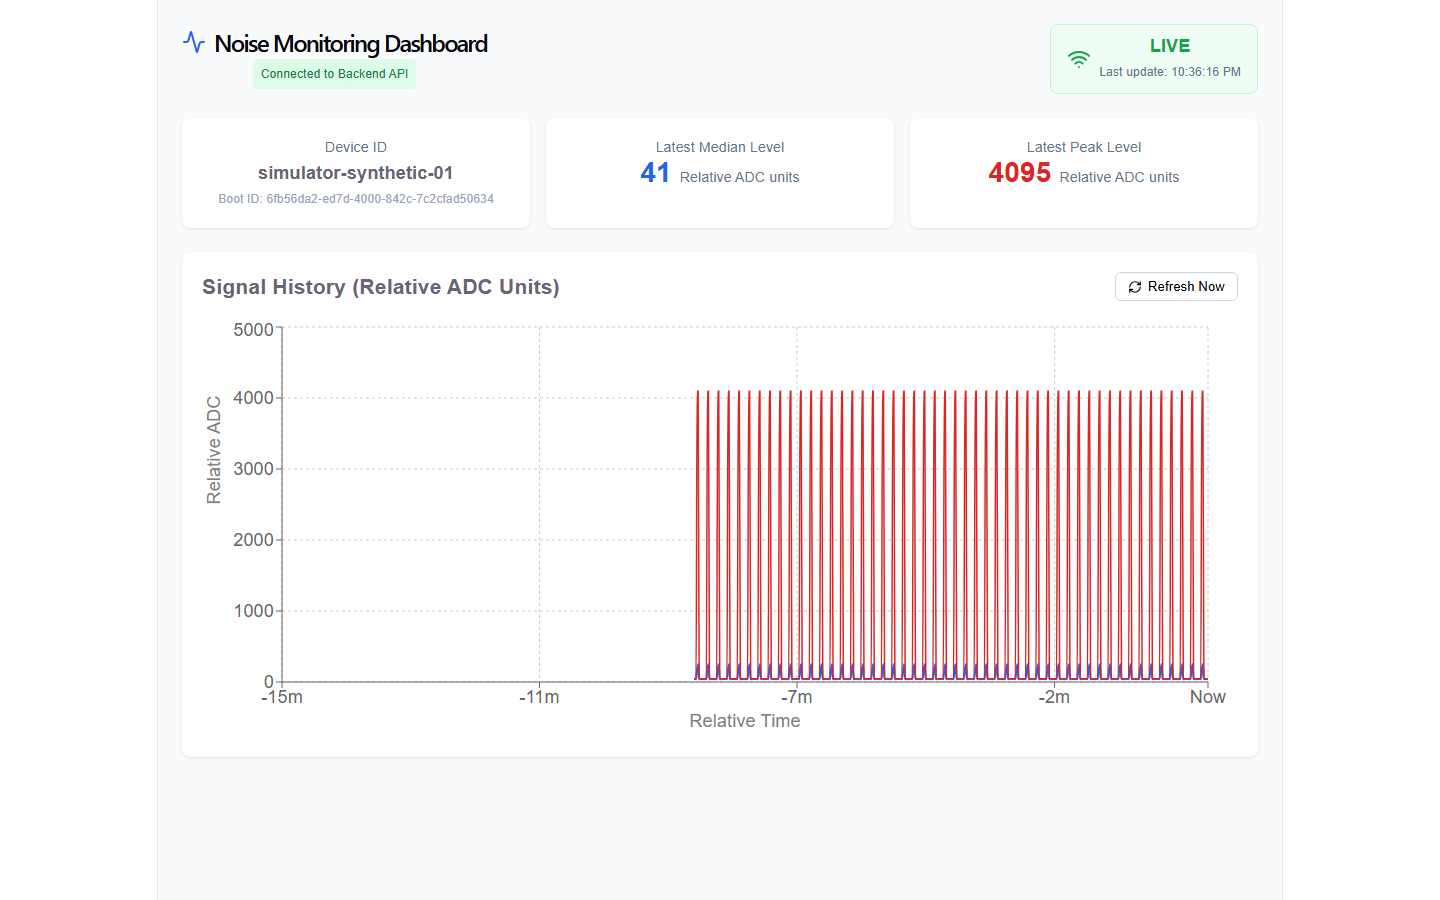
\includegraphics[height=4.0cm, trim=157 130 157 0, clip]{figures/demo-4-dashboard-live.png}}\\[1mm]
      {\footnotesize LIVE · trung vị 41 · đỉnh 4095 (bão hòa ADC)}
    \end{column}
    \begin{column}{0.49\textwidth}
      \centering
      \termlabel{\cnum{4} Ngừng gửi > 30 giây}
      \fbox{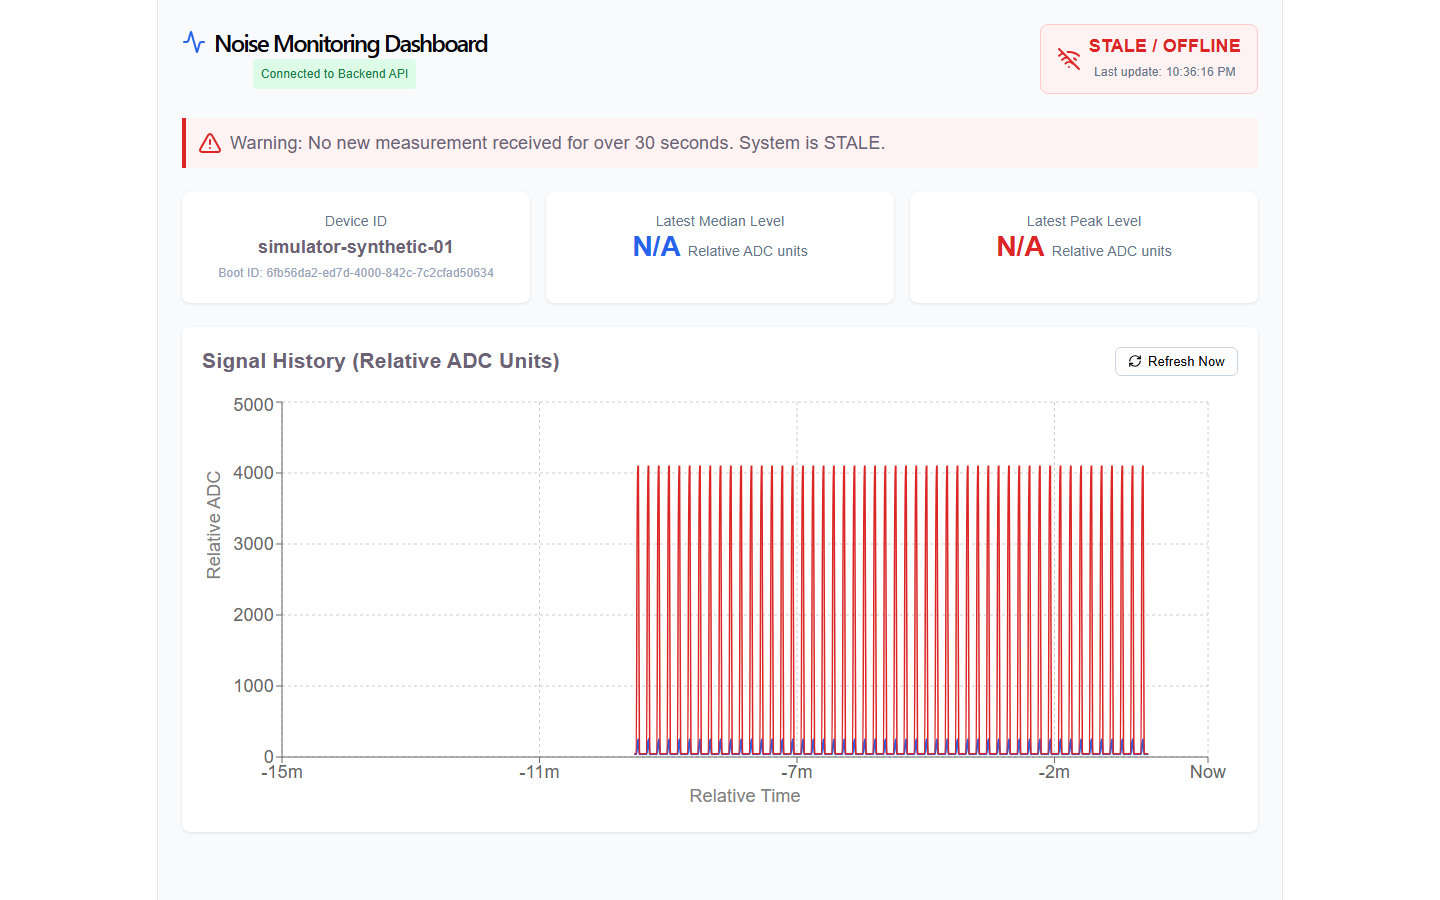
\includegraphics[height=4.0cm, trim=157 55 157 0, clip]{figures/demo-5-dashboard-stale.png}}\\[1mm]
      {\footnotesize \textcolor{warn}{\textbf{STALE / OFFLINE}} · mức hiện tại N/A}
    \end{column}
  \end{columns}

  \vspace{1.2mm}
  {\scriptsize\textit{Cùng lần chạy và boot\_id với trang trước.} \textcolor{warn}{\textbf{Dữ liệu giả lập.}}}
\end{frame}

\begin{frame}{Khó khăn và bước tiếp theo}
  \scriptsize
  \begin{columns}[T]
    \begin{column}{0.52\textwidth}
      \begin{alertblock}{Khó khăn}
        \footnotesize
        \begin{enumerate}\setlength{\itemsep}{1pt}
          \item Chưa có phần cứng: firmware chưa kiểm chứng thực tế, chưa chọn được gain và ngưỡng.
          \item P2P là đơn vị tương đối, chưa hiệu chuẩn sang dB: phải đo thực nghiệm trong phòng để đặt ngưỡng ``ồn''.
          \item ESP32 không có đồng hồ thời gian thực: cần đồng bộ thời gian (NTP) để gán đúng thời điểm đo.
          \item Mất mạng: hiện gói lỗi bị bỏ, chưa gửi bù (Sprint 3).
        \end{enumerate}
      \end{alertblock}
    \end{column}
    \begin{column}{0.46\textwidth}
      \begin{block}{Bước tiếp theo}
        \footnotesize
        \begin{enumerate}\setlength{\itemsep}{1pt}
          \item Mua linh kiện, nạp firmware, kiểm tra phản ứng với âm thanh thật.
          \item Chạy thử $\geq$ 30 phút trên phần cứng, đo độ trễ (\#7).
          \item Sprint 2: ngưỡng 30 giây, LED, sự kiện, báo cáo đêm.
        \end{enumerate}
      \end{block}
    \end{column}
  \end{columns}
\end{frame}

\hustcontactpage{\hfill Nhóm 14 · PAN \hfill}{
  \textbf{Repo:} \url{https://github.com/nnta301/noise-monitor}\\
  \vspace{1cm}
  \textit{Xin cảm ơn thầy và các bạn đã lắng nghe!}
}

\hustthankyou

\end{document}
